\documentclass[twocolumn]{article}
\usepackage[utf8]{inputenc}
\usepackage{multicol}
\usepackage{graphicx}
\usepackage[12pt,a4paper, total={6.4in,10.5in}]{geometry}
\usepackage{float}
\usepackage{enumitem}
\usepackage{algorithmic}
\usepackage{caption}
\usepackage{amsmath}
\usepackage{algorithm}

\title{Continuous mapping of Rey-Osterrieth complex figure test using Variational Autoencoders}
\author{Matías Grinberg}
\date{January 2019}

\begin{document}
\maketitle 
\section{Abstract}
Deep neural networks were used to develop a scoring system for the Rey-Osterrieth complex figure test. Empirical results are contrasted with  patient data to account for external validity. 
The mapping of each observation to the generated latent vector space allows for new kinds of analysis which were previously unreacheable using traditional methodology, with the added benefit of automation. 

\section{Introduction}
The advent of neural networks has conveyed previously unimagined possibilities in most of human intellectual endeavours.  This method's capacity is increasing exponentially, demonstrating new state of the art advancements every few weeks. In health, it will in many cases cause the evolution from categorical classifications systems to ones of continuous or dimensional representation as has been suggested in %DSM
.This linking of nosologic entities in an abstract space allows for applications in both diagnosis and rehabilitation. 

The Rey–Osterrieth complex figure test (ROCF) is a widely used neuropsychological assessment in which subjects are asked to copy a line drawing under three conditions: Copy, Immediate Recall and Delayed Recall. The performance depends on many distinct cognitive capacities, serving as an evaluation of visuospatial abilities, memory, attention, and executive functions.

\begin{figure} [H]
    \centering
    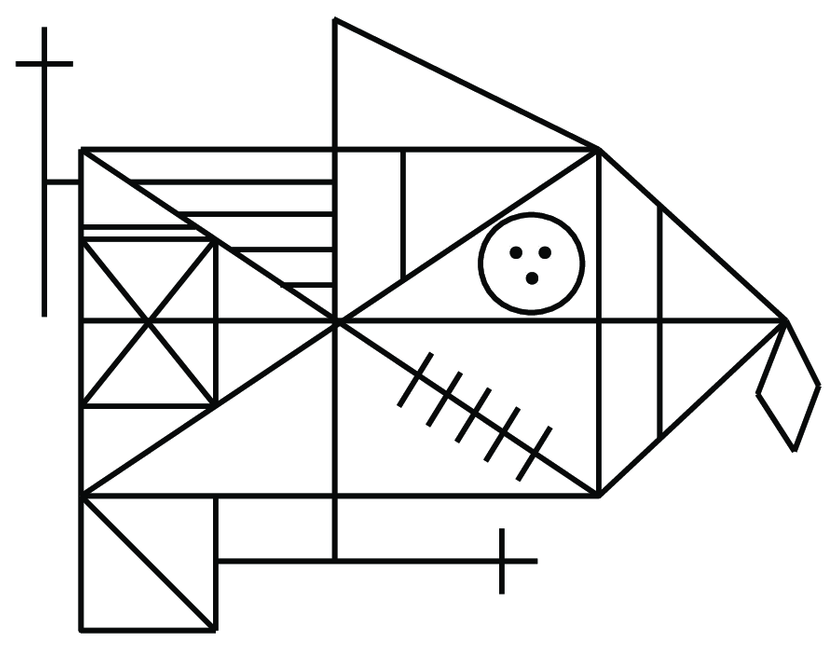
\includegraphics[scale=0.15]{ROCF.png}
    \caption{Rey-Osterrieth Complex Figure}
    \label{fig:aes}
\end{figure}

% SCORING SYSTEMS
Traditionally, scoring systems such as Boston \cite{8} rely on subjective appreciation of the accuracy of the drawing, manually grading each listed element..  
% Continuous latent space VAEs

\section{Neuropsychology}

\subsection{Cognitive correlates}

For both clinical and research settings, the ROCF is used to examine visual spatial constructional ability, nonverbal memory skills and executive functioning \cite{1}. It has been theorized or shown to measure various cognitive dimensions, including problem and planning solving strategies %% -acá hay mas (en cita)- 
\cite{2} attention and concentration levels, fine-motor coordination, and organizational skills \cite{6}.

%% Memory (un parrafito por cada una)
%% Attention
%% Visuospatial
%% Motor / others

\subsection{Neurobiological correlates}
%% Idem pero neurobio
The ROCF is considered to be a useful tool for the
evaluation of frontal lobe function, which is required for strategic
planning and organizing \cite{3}

%ESPECIFICAR

\subsection{Current usage}
%% Difusion de la herramienta
%% Use in diagnostics

There are characteristic ways to perform the task associated with different types of brain injury. 
ROCF has been used to assess visual memory disturbance and recall deficits in individuals with schizophrenia \cite{4, 5} and in patients with traumatic brain injury and individuals with aneurysms of the anterior communicating artery \cite{6}. Patients with right-hemisphere damage tend to do more poorly than do left hemisphere-damaged patients, even though both
groups present significant numbers of errors. Poor performance on this test has been found in patients with different localization of focal damage. Also, individuals with Alzheimer’s disease (AD), Huntington’s disease (HD), and Korsakoff’s syndrome have shown poorer copy and recognition on the ROCF than controls \cite{2}.


\subsection{Population Parameters}
%% Types of patients and profiles
A considerable number of studies have measured ROCF performance in a variety of locations and sample characteristics. A meta-analytic review is beyond the scope of this work, but a few important statistics are taken for reference.

%% Classification metrics for different conditions
%% Normal variability within neurotypical group
%% Difference between pathological groups
% igual no se que tan buena data hay ni cuanto va a servir, dejalo para lo ultimo! no?

The performance in ROCF is affected by age, education, and gender \cite{7}


\section{Deep Learning}

Machine learning methods consist on algorithms that given training data, improve with the optimization of some objective function. In contrast with "shallow" machine learning, neural networks rely on layers of unitary parts or "neurons" that, most generally, apply a linear combination on the input and a non-linearity. This allows for discrete transformations of the input manifold that, if successful, render the problem linearly approximable. Differentiating the loss function with respect to each coefficient of the network with a \textit{backpropagating} fashion, gradient descent is used to \textit{train} the weights of network using batches of data. 

%\subsection{Neural Networks}

\subsection{Data}
From a small group of example drawings, we construct a ROCF generator that provides unlimited samples to build an initial latent space. Direct manipulation of the variability of the training dataset is useful to approximate the expected generative distribution, and it permits non-random training schemes such as curriculum or skill-specific training.
To generate the data, we first sample drawn polygons from ROCF examples. To detect polygons, the process consists of:
\begin{enumerate}
\item[--] Filtering

    Scharr filter 
\item[--] Contour finding

    Thresh otsu
\item[--] Polygon Approximation

    Remove redundant 
\item[--] Thresholding

    Otsu
\end{enumerate}


A generator function was used to sample from that set, feeding the neural network after a data augmentation pipeline. To account for possible variability, many augmentation layers where applied to each polygon group sampled.

\begin{algorithm}
\caption{Data Generation Pipeline}
\label{datagen}
    \begin{algorithmic}
    \STATE Initialize blank image
    \FOR{random layers}
        \STATE Sample $p$ polygons
        \STATE Add augmentations(polygons) to image
    \ENDFOR 
    
\end{algorithmic}
\end{algorithm}


\subsection{VAEs}
%Autoencoders
%Variational Autoencoders

\begin{figure} [H]
    \centering
    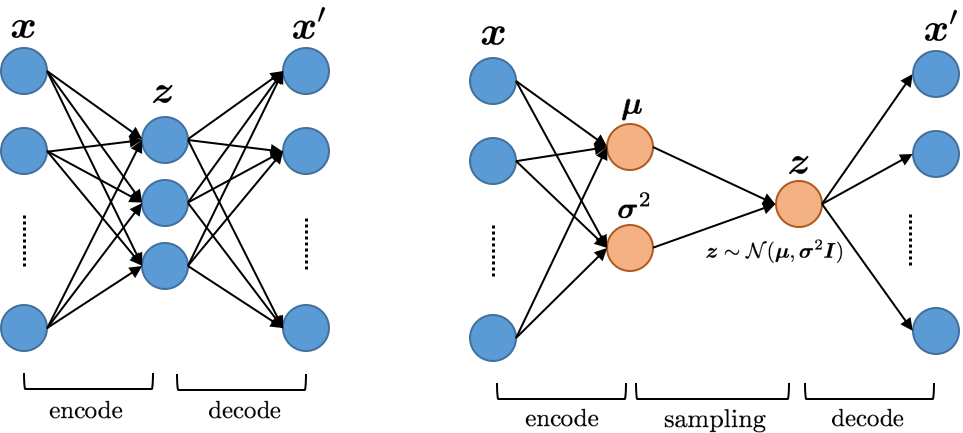
\includegraphics[scale=0.15]{aes.png}
    \caption{Autoencoders. Left: regular, right: variational}
    \label{fig:aes}
\end{figure}

% Architecture
% Training

\section{Results}

\subsection{External Validation}

\subsection{Discussion}


\begin{thebibliography}{X}
\bibitem{1}
Somervile, J., Tremont, G. & Stern, R.A. (2000). The Boston Qualitative Scoring System as a measure of executive functioning in
Rey–Osterrieth Complex Figure performance. Journal of Clinical
and Experimental Neuropsychology, 22(5), 613-621.

\bibitem{2}
Lezak, M. D., Howieson, D. B., & Loring, D. W. (2012). Neuropsychological assessment (5th ed.). New York: Oxford University
Press

\bibitem{3}
Shin, M.-S., Kim, Y.-H., Cho, S.-C., & Kim, B.-N. (2003). Neuropsychologic Characteristics of Children with Attention-Deficit Hyperactivity Disorder (ADHD), Learning Disorder, and Tic Disorder on the Rey-Osterreith Complex Figure. Journal of Child Neurology, 18(12), 835–844. 

\bibitem{4}
Calev, A., Edelist, S., Kugelmass, S., & Lerer, B. (1991). Performance
of long-stay schizophrenics on matched verbal and visuospatial
recall tasks. Psychological Medicine, 21(3), 655-660

\bibitem{5}
Silverstein S. M., Osborn L. M., & Palumbo D. R. (1998). ReyOsterrieth Complex Figure test Perfomance in Acute, Chronic,
and Remitted Schizophrenia Patients. Journal of Clinical Psychology, 54(7), 985-994.

\bibitem{6} 
Rivera D, Perrin PB, Morlett-Paredes A, Galarza-Del-Angel J, Martínez C, Garza
MT, Saracho CP, Rodríguez W, Rodríguez-Agudelo Y, Rábago B, Aliaga A, Schebela S, Luna M, Longoni M, Ocampo-Barba N, Fernández E, Esenarro L, García-Egan P,Arango-Lasprilla JC (2015). Rey-Osterrieth Complex Figure - copy and immediate recall: Normative data for the Latin American Spanish speaking adult population.
NeuroRehabilitation. 2015;37(4):677-98


\bibitem{7}
Roselli, M. & Ardila, A. (1991). Effects of age, education, and gender
on the Rey-Osterrieth Complex Figure. The Clinical Neuropsychologist, 5(4), 371-376.

\bibitem{8}
Stern, R. A., Singer, E. A., Duke, L. M., Singer, N. G., Morey, C. E., Daughtrey, E. W., & Kaplan, E. (1994). The Boston qualitative scoring system for the Rey-Osterrieth complex figure: description and interrater reliability. The Clinical Neuropsychologist, 8(3), 309-322.

\end{thebibliography}
\end{document}
